%*******************************************************************************
% * Copyright (c) 2006-2013 
% * Institute of Automation, Dresden University of Technology
% * 
% * All rights reserved. This program and the accompanying materials
% * are made available under the terms of the Eclipse Public License v1.0 
% * which accompanies this distribution, and is available at
% * http://www.eclipse.org/legal/epl-v10.html
% * 
% * Contributors:
% *   Institute of Automation - TU Dresden, Germany 
% *      - initial API and implementation
% ******************************************************************************/

\documentclass[
%  print,          % print optimized version of the thesis, standard option
                  % alternative:
  screen,        % makes the thesis better readable on screens (onesided, coloured links)
                  % use only 'print' OR 'screen'
                  % ATTENTION: 'screen' changes size of text area slightly. Always optimize document WITH
                  % 'print' option first for printing (size of graphics etc.) and convert afterwards
                  % in screen optimized version!
  %listoffigures,  % includes list of figures
  %listoftables,   % includes list of tables
  %listoflistings, % includes list of listings
  abbrevations,   % includes index of symbols and abbrevations
  bibIfa,         % citation style (IfA standard), alternatives: bibNumeric, bibHarvard
  biber,          % bibliography backend, alternatives: bibtex, bibtex8, biber
  langDE         % define the language (default: langDE)
%  noIfaLogo,     % prevents the 'IfA' logo from being inculded in the header for the title page and abstract
%  a5paper        % switches to 'A5' paper size (this may only be used for Dissertations!!!)
]{ifathesis}

%***********************************
% General commands
%***********************************

\ifaThesis{Dokumentation}                               % type of the thesis                
\ifaAuthor{Max Kirchner}                            % author of the thesis
\ifaAuthorBirthday{03.05.1998}                         % date of birth
\ifaAuthorBirthplace{Räckelwitz}             % place of birth
\ifaAuthorCourse{Elektrotechnik}                          % study program
\ifaAuthorYearOfMatriculation{2017}                    % year of immatriculation
\ifaKeywords{Dokumentation, Hauptseminar AMR, Robotik, Einparkhilfe}    % Keywords included in pdf-file. Could be found e.g. by Windows file search.
\ifaTitleDE{Hauptseminar Automatisierungs-, Mess- und Regelungstechnik}       % geman title of the thesis
%\ifaTitleEN{Teleautomation, Chances and Risks}         % english title of the thesis
%\ifaAbstractDE{example_files/00_abstract_de}           % a tex file containing the german abstract
%\ifaAbstractEN{example_files/00_abstract_en__invalid}  % a tex file containing the german abstract
%\ifaAbbrev{}                                          % a tex file containing the various abbreviations to include into the list of abbreviations (alternatively,
%\ifaUserListings{}                                    % a tex file containing additional listings to be printed (besides list of figures, tables, and/or listings)
%\ifaAcknowledegments{}                                % the acknowlegements for the thesis (usually only used for dissertation)
                                                       % these may also be defined in the text where they are first used)

% supervisors of the thesis (for dissertations, this can be used to indicate the reviewers)
\ifaSupervisorA{Dr.-Ing. Carsten Knoll}
\ifaSupervisorB{Dipl.-Ing. Elias Scharf}
\ifaSupervisorC{Dipl.-Ing. Julian Rahm}
\ifaSupervisorD{Dr.-Ing. Andrey Morozov}
\ifaSupervisorE{Dipl.-Ing. Mustafa Saraoglu}

\ifaProfessor{Prof. Dr. techn. Klaus Janschek}         % supervising professor as indicated on the topic description
\ifaDayOfSubmission{12.01.2020}                        % the day the thesis is submitted
%\ifaTopicDescriptionPDF{example_files/00_Aufgabenstellung.pdf} % a PDF file of the topic description
%\ifaAppendix{example_files/appendix}                   % a tex file containing the appendix for the thesis

% Literaturverzeichnis angeben
\bibliography{bibliography}                            % a bib file containing the reference sources
\ifaBibliographyBeforeAppendix{false}	                 % print the bibliography before or after the appendix ('true' or 'false')
%\ifaAdditionalContributors{}                           % additional contributors to be included in the statement of authorship

%***********************************
% Special commands for dissertations
%***********************************

%\ifaDissertationStage{Gutachten}                      % stage of the dissertation ('Gutachten' or 'Pflichtexemplare')
%\ifaChair{}                                           % chair of the phd board
%\ifaDayOfDefense{}                                    % the day the dissertation was defended (only used in 'Pflichtexemplare' mode)
%\ifaIncludeBeforeTitlePage{}                          % include additional content before the title page (e.g. bastard title or impressum)
%\ifaIncludeAfterTitlePage{}                           % include additional content between title page and abstract (e.g. impressum or dedication)
%\ifaCV{}                                              % include a CV at the end of the document
%\ifaIncludeAtEndOfDocument{}                          % include additional content at the end of the document (e.g. to reach an even number of pages)


%***********************************
% The actual content of the thesis
%***********************************

\begin{document} 
\chapter{Analyse der Aufgabenstellung}


\section{Allgemeine Funktionsbeschreibung und Ziele}

Das Ziel des Moduls Guidance (deutsch Führung) ist die anderen Module miteinander zu verbinden und sie zu steuern. 
Damit dies möglich ist, wurde mit den Modulverantwortlichen alle Funktionalitäten besprochen. \\

\noindent Die Hauptfunktion des Roboters ist das Abfahren eines Parcours. Dabei wird nach passenden Parklücken gesucht. Dieser Zustand heißt Scout-Modus.
In eine der gefundenen Lücken soll anschließend eingeparkt werden. Mit Hilfe einer Android-App werden Steuersignale übermittelt. Wenn zum Beispiel das Ausparksignal übertragen wird, folgt der Roboter einem Polynom und wechselt anschließend in den Scout-Modus. Gefordert ist zusätzlich, dass von jeder Aktion das Fahrzeug in einen Pause-Modus gewechselt werden kann.

\section{Geplantes Vorgehen}

Um den Missionsplaner und Pfadgenerator zeit effektiv zu implementieren, wurde als erster Schritt eine theoretische Vorbetrachtung getätigt. Dabei wurde ein Zustandsdiagramm mit entsprechenden Aktionstabellen und die Berechnungsvorschrift für das Pfadpolynom entworfen. \\
\noindent Für den Entwurf der Zustandsmaschine wurde die Onlinesoftware Lucidchart verwendet. Mit dieser ist es möglich Diagramme zu zeichnen. \\

\noindent Anschließend wurden die Modelle implementiert. Beim Programmieren sollte regelmäßig der aktuelle Stand in ein \glqq GitHub Repository\grqq{} geladen werden, damit die anderen Module ihre Funktionen testen können.

\section{Schnittstellen und Zusammenarbeit zu/mit anderen Modulen/Modulverantwortlichen}

Das Projekt wurde in der objektorientierten Programmiersprache Java umgesetzt. Dies ermöglicht eine klare Modultrennung. Damit unsere Gruppe eine Versionsverwaltung besitzt, entschieden wir uns für ein \glqq GitHub Repository\grqq{}.\\


\noindent Mit Hilfe von Setter-Methoden ist es möglich festzulegen, welche Funktionen in den entsprechenden Modulen ausgeführt werden sollen.
Im Gegenzug können mit Getter-Methoden aktuelle Eigenschaften des Roboters abgefragt werden. Mit diesen Informationen werden die jeweiligen Zustandsübergänge überprüft.\\

\noindent Unsere Gruppe hat sich regelmäßig getroffen. Dabei wurden Etappenziele gesetzt und wichtige Änderung besprochen. Zum Beispiel sollte bis Ende 2019 alles implementiert sein, damit in den letzten zwei Wochen ein ausführlicher Funktionstest durchgeführt werden kann und alle auftretenden Fehler beseitigt werden können.\\

\noindent Beim Programmieren war es auch oft notwendig zusammen zu arbeiten, weil man allein nicht alles überschauen konnte. Vor allem die Demoprogramme zwei und drei wurden zusammen mit der Control implementiert. Ich programmierte alle notwendigen Methodenaufrufe und Zustandswechsel. Der Controlverantwortliche konnte seine Regler testen und anpassen, sodass alle Manöver abfahrbar waren.\\

\noindent Durch die Implementierung der Demoprogramme war es möglich einen guten Überblick über die Programmteile der anderen Module zu bekommen. Es ist somit möglich mein Programmentwurf stückweise zu testen. Auftretende Fehler in allen Modulen konnten entdeckt werden. Vor allem jene, die erst beim Zusammenspiel mit allen Modulen auftraten. Durch die Zusammenarbeit wurden diese schnell behoben. 
\chapter{Entwurf Missionsplaner}

\section{Geforderte Funktionen}

Die geforderten Funktionen können in fünf Kategorien eingeteilt werden.
\renewcommand{\labelenumi}{\roman{enumi}}
\begin{enumerate}
\item 	Scout-Modus mit Parklückensuche
\item 	Einparken
\item	Parken
\item	Ausparken
\item	Inaktiv sein
\end{enumerate}

\noindent Diese Kategorien definieren die Hauptzustände.\\

\noindent Was das Fahrzeug in jener Kategorie machen soll, ist in den Unterzuständen definiert.\\


\noindent Scout-Modus bedeutet, dass das Fahrzeug einen Parcours abfährt. Dabei wird einer Linie gefolgt. Wenn eine Ecke detektiert wird, muss die Geschwindigkeit reduziert werden. Das Ziel dabei ist, dass die Regelung genauer arbeiten kann und die Kurve abgefahren wird. Während dem Abfahren sucht der Roboter nach Parklücken.\\

\noindent In dem Zustand \glqq Park\_This\grqq{} wird als erstes die Startpose angefahren. Danach wird ein Polynom abgefahren. Wenn die Zielpose in der Lücke erreicht ist, wechselt der Automat automatisch in den Zustand \glqq Park\grqq{}. In diesem wird gewartet, bis über die App das Ausparksignal übermittelt wird.\\

\noindent Beim Ausparken folgt der Roboter erneut einem Polynom zurück auf die Linie. Dabei muss sichergestellt werden, dass nach vorne genügen Freiraum vorhanden ist, sonst gibt es einen Unfall mit der Bande.\\

\noindent Vor allem für das Ein - und Ausparken müssen neben den Hauptzuständen die jeweiligen Unterzustände abgespeichert werden, damit beim Fortsetzen die richtigen Aktionen ausgeführt werden. Bei den Abfahrtspolynomen muss beachtet werden, dass kein neues Polynom berechnet wird. 



\section{Hauptzustandsmaschine}

Für den Entwurf der folgenden Zustandsmaschinen wurde sich an den geforderten Funktionen orientiert. Dabei wurde beachtet, dass die Aufteilung so getätigt wird, dass die Zustandsübergange möglichst einfach sind.\\

\noindent \begin{tabular}{|p{1.5cm}|p{4cm}|p{3.8cm}|p{3cm}|}
	\hline 
	Zustand & Eingangsaktion & Nominalaktion & Ausgangsaktion \\ 
	\hline 
	Driving & Auswahl des Controlmodus & siehe Unterzustandsmaschine & Parklückensuche ausschalten \\ 
	\hline 
	 & Parklückensuche einschalten (Ausnahme bei der Anfahrt) &  &  \\ 
	\hline
	Inactive & Setzen des Controlmodus \glqq INACTIVE\grqq{} & siehe Unterzustandsmaschine &  \\ 
	\hline 
	& Abspeichern des Vorzustandes & &  \\ 
	\hline 
	Exit &  & Abschalten des Systems &  \\ 
	\hline
	Park & Auswahl Controlmodus \glqq INACTIVE\grqq & Ausgabe Sensordaten (Abstand nach vorn und hinten, Position) &  \\ 
	\hline
	Park This & Auswahl des richtigen Subzustandes & siehe Unterzustandsmaschine &  \\ 
	\hline
	 & Parkplatzinformation abfragen &  &  \\ 
	\hline
	 & Variable \glqq anfahrt\grqq und \glqq correct\grqq auf falsch setzen &  &  \\
	\hline
	Park Out & Auswahl des richtigen Subzustands & siehe Unterzustandsmaschine &  \\ 
	\hline 
	 & 	Variable \glqq back\grqq & & \\
	\hline
\end{tabular} 

\begin{figure}[h]
	\centering
	\includegraphics[width=0.9\textwidth]{Zustandsautomataußen}
	\caption{Entwurf Hauptzustandsautomat}
	\label{img:grafik-Hauptzustandsautomat}
\end{figure}

\section{Unterzustandsmaschine}

\subsection{Scout-Modus}

\begin{tabular}{|p{1.5cm}|p{4cm}|p{4cm}|p{3cm}|}
	\hline 
	Zustand & Eingangsaktion & Nominalaktion & Ausgangsaktion \\ 
	\hline 
	Slow & Controlmodusauswahl \glqq SLOW\grqq  &  &  \\ 
	\hline 
	Fast & Controlmodusauswahl \glqq FAST\grqq  &  &  \\ 
	\hline 
\end{tabular} 

\subsection{Pause}

Es gibt keine Unterzustandsmaschine.

\subsection{Exit}

Es gibt keine Unterzustandsmaschine.

\subsection{Park}

Es gibt keine Unterzustandsmaschine.

\subsection{Park This}

\begin{tabular}{|p{1.5cm}|p{4cm}|p{4cm}|p{3cm}|}
	\hline 
	Zustand & Eingangsaktion & Nominalaktion & Ausgangsaktion \\ 
	\hline 
	To Slot & Zielwinkelberechnung & Zustand \glqq DRIVING\grqq bis Pose erreicht ist &  \\ 
	\hline 
	 & Anfahrort festlegen &  &  \\ 
	\hline
	Reached Slot & Start- und Endpose vom Polynom festlegen &  &  \\ 
	\hline
	 & Geschwindigkeit festlegen &  &  \\ 
	\hline 
	 & Setzen des Controlmodus \glqq PARK\_CTRL\grqq   & Überprüfung ob Polynom abgefahren wurde &  \\ 
	\hline
	In Slot &  & Variable \glqq back\grqq  auf wahr setzen &  \\ 
	\hline 
	
\end{tabular} 

\subsection{Park Out}

\begin{tabular}{|p{1.7cm}|p{4cm}|p{4cm}|p{3cm}|}
	\hline 
	Zustand & Eingangsaktion & Nominalaktion & Ausgangsaktion \\ 
	\hline 
	Backwarts & Berechnung der Rückfahrdistanz & Überprüfung ob das Zurückfahren erfolgt ist &  \\ 
	\hline
	 & Setzen des Controlmodus \glqq SETPOSE\grqq & &\\ 
	\hline
	ParkOut & Start- und Endpose vom Polynom festlegen  & Überprüfung ob Polynom abgefahren wurde  &  \\ 
	\hline 
	 & Geschwindigkeit festlegen  &  &  \\ 
	\hline  
	& Setzen des Controlmodus \glqq PARK\_CTRL\grqq & &  \\ 
	\hline
 
\end{tabular} 

\begin{figure}[h]
	\centering
	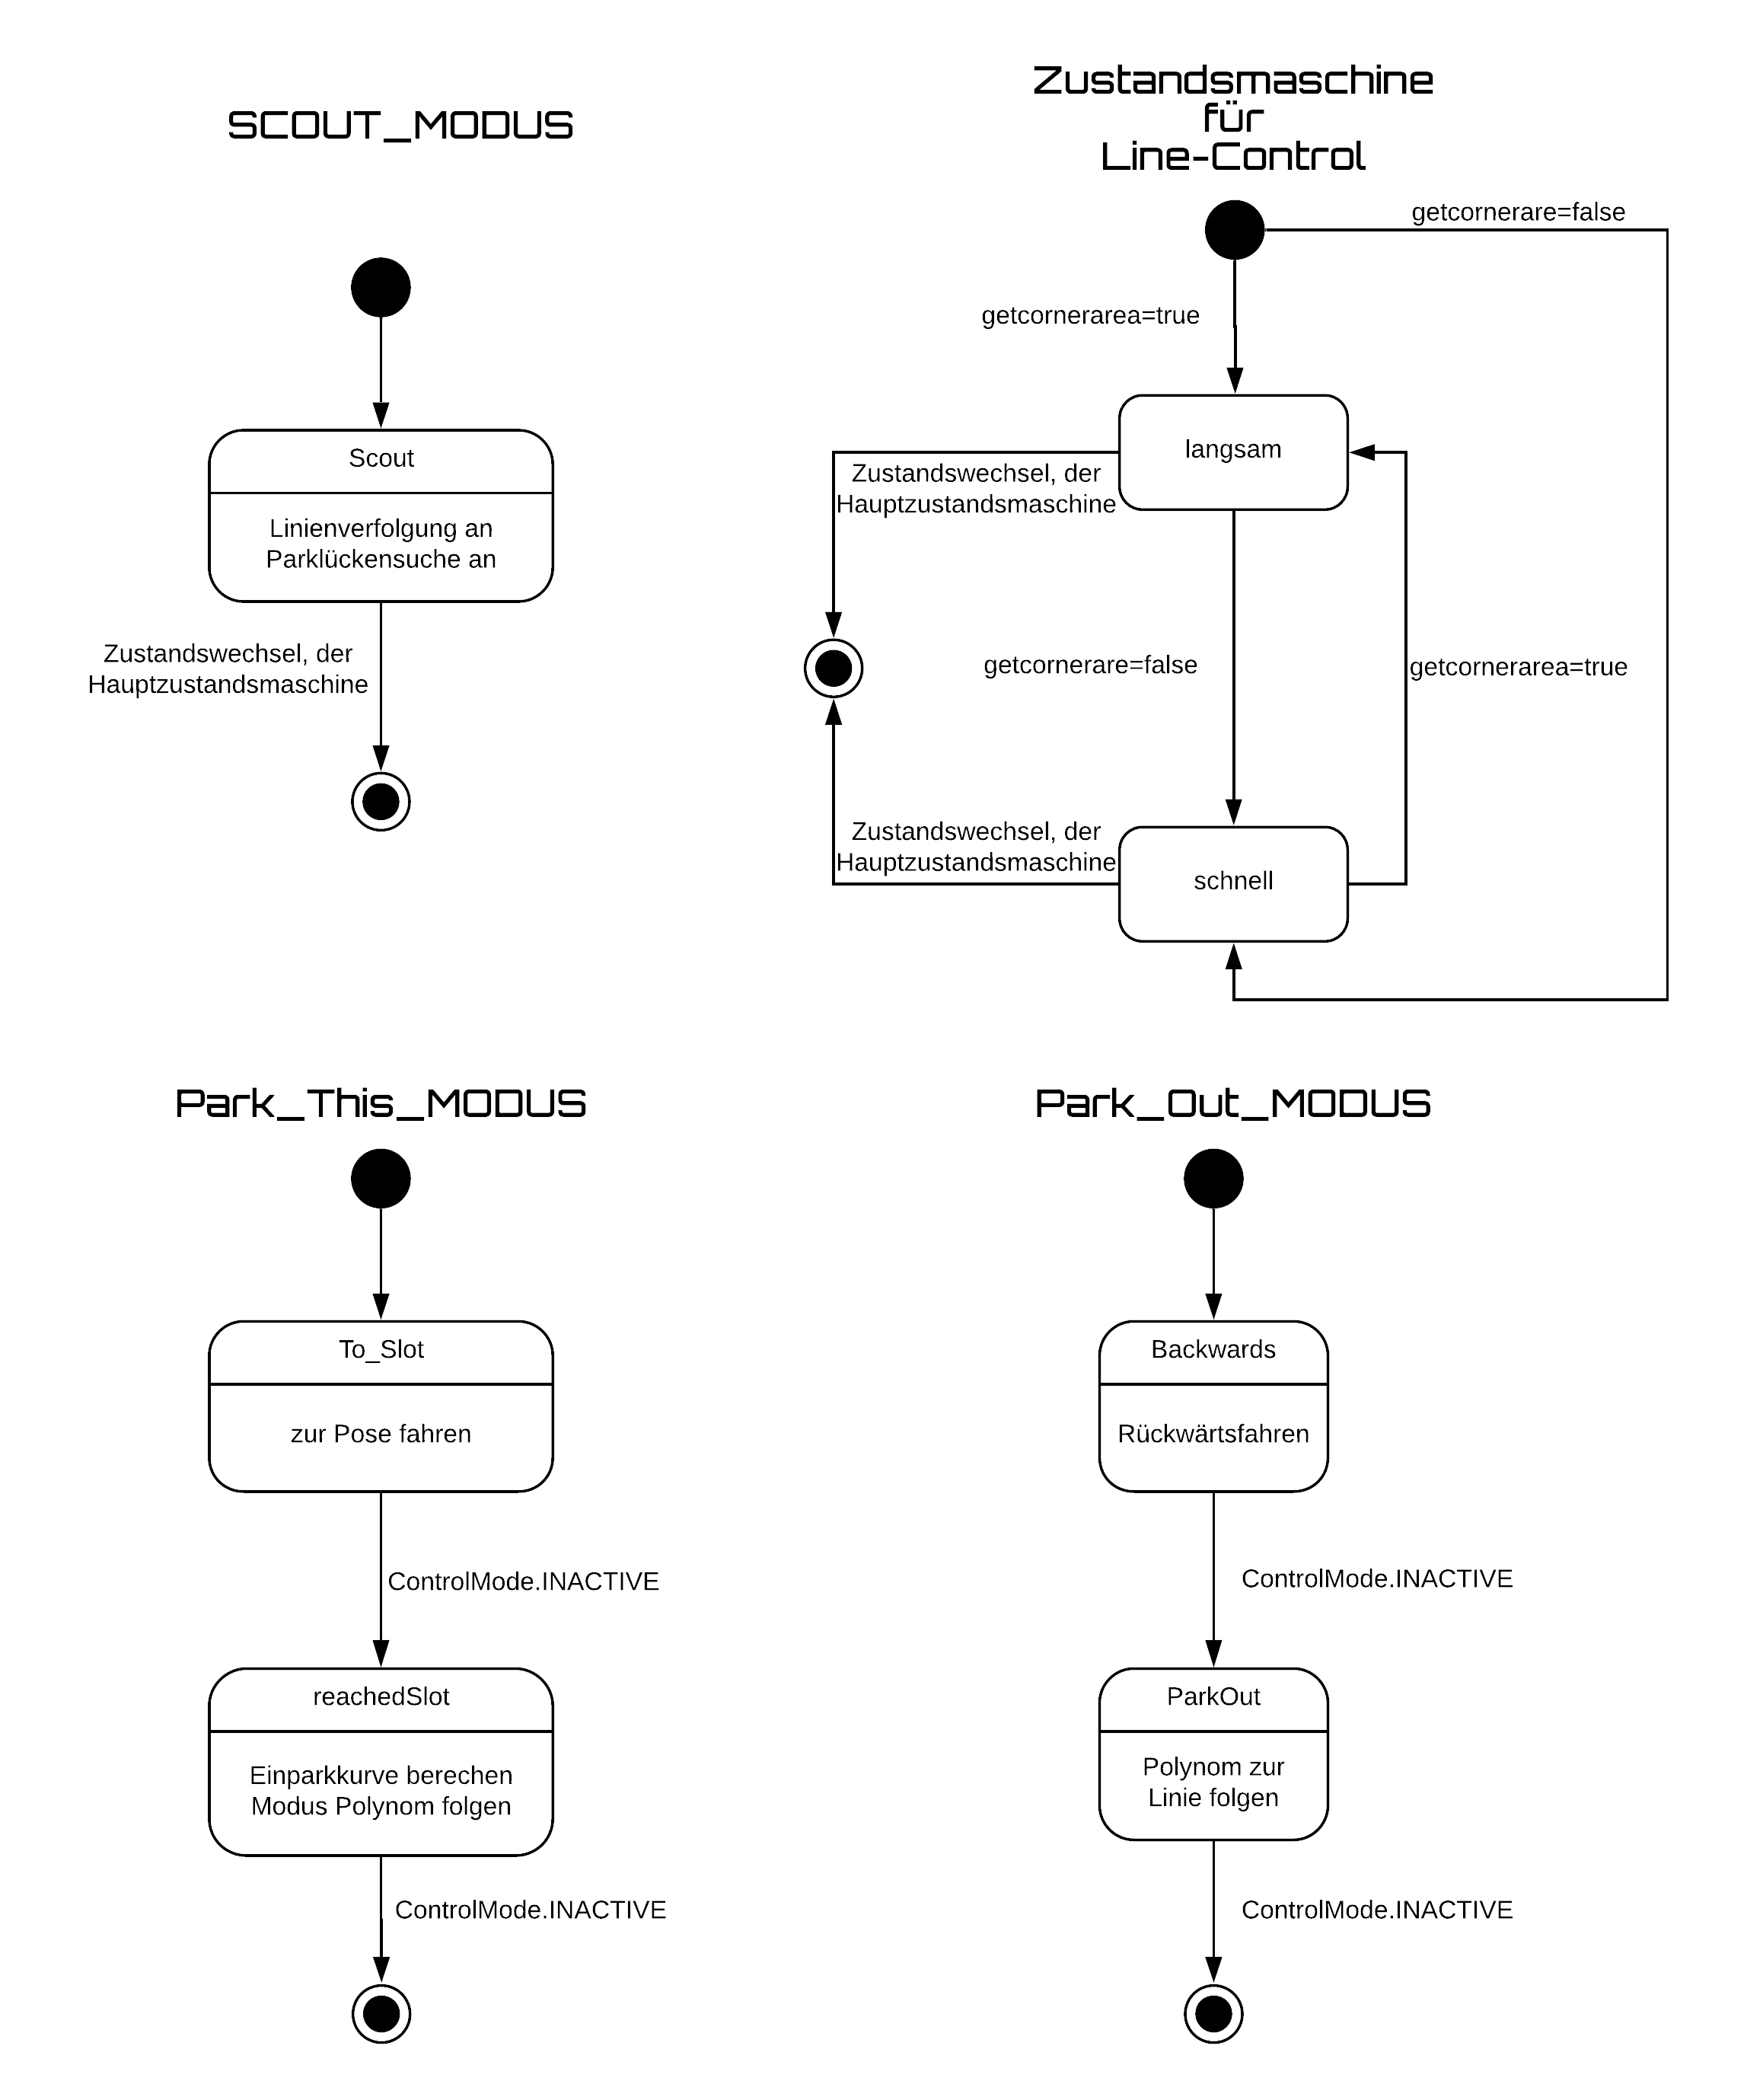
\includegraphics[width=0.9\textwidth]{Subzustandsmaschine}
	\caption{Entwurf Unterzustandsmaschine}
	\label{img:grafik-Unterzustandsautomat}
\end{figure}

\chapter{Entwurf Pfadgenerator}

\section{Geforderte Funktionen}

Damit der Roboter einparken kann, muss er einem Polynom folgen. Dabei ist zu beachten, dass für jede Parklücke individuell ein Polynom entwickelt werden muss.\\

\noindent In dem Modul Guidance wird die Start- und Endpose festgelegt. Anschließend muss der entsprechende Controlmodus gestartet werden. Die Berechnung des Polynoms wird danach im Control-Modul aufgerufen. 


\section{Mathematische Beschreibung}

Eine einfache und gute Einparkkurve entspricht einer Funktion dritten Grades:
\begin{equation}
f=y(x)=a*x^3+c*x^2+b*x+d
\end{equation}

\noindent Die Funktion soll durch den Koordinatenursprung gehen ($ d=0 $) und punktsymmetrisch sein (nur ungerade Exponenten $ \Rightarrow c=0 $). 

\noindent Das Problem vereinfacht sich auf folgendes Polynom:

\begin{equation}
f=y(x)=a*x^3+b*x
\end{equation}

\noindent Es werden zwei Bedingungen benötigt, damit die Koeffizienten berechnet werden können. 

\begin{equation}
 y'_{ende}=f'(x_{ende})=3*a*x_{ende}^2+b=0
 \end{equation}
 \begin{equation}
y_{ende}=a*x_{ende}^3+b*x_{ende}
 \end{equation}
 
\noindent Durch das Umstellen folgt:
 %this.trajectory_a = endPose.getY()/(-2*Math.pow(endPose.getX(),3));
 \begin{equation}
a=-\dfrac{y_{ende}}{2*x_{ende}^3}
\end{equation}
\noindent und
%this.trajectory_c = -this.trajectory_a*3*Math.pow(endPose.getX(),2);
\begin{equation} 
b=-3*a*x_{ende}^3
\end{equation}

\noindent Damit die Brechung stets auf das selbe Problem zurückzuführen ist, gibt es einen globales und lokales Koordinatensystem. Wie in der Abbildung \ref{img:grafik-Parkluecke} zu sehen, ist der Mittelpunkt zwischen Start- und Zielpose im globalen Koordinatensystem identisch mit dem Ursprung des lokalem Systems. Dieses ist je nach Richtungswinkel des Roboters entsprechend gedreht. \\
   
\begin{figure}[h]
	\centering
	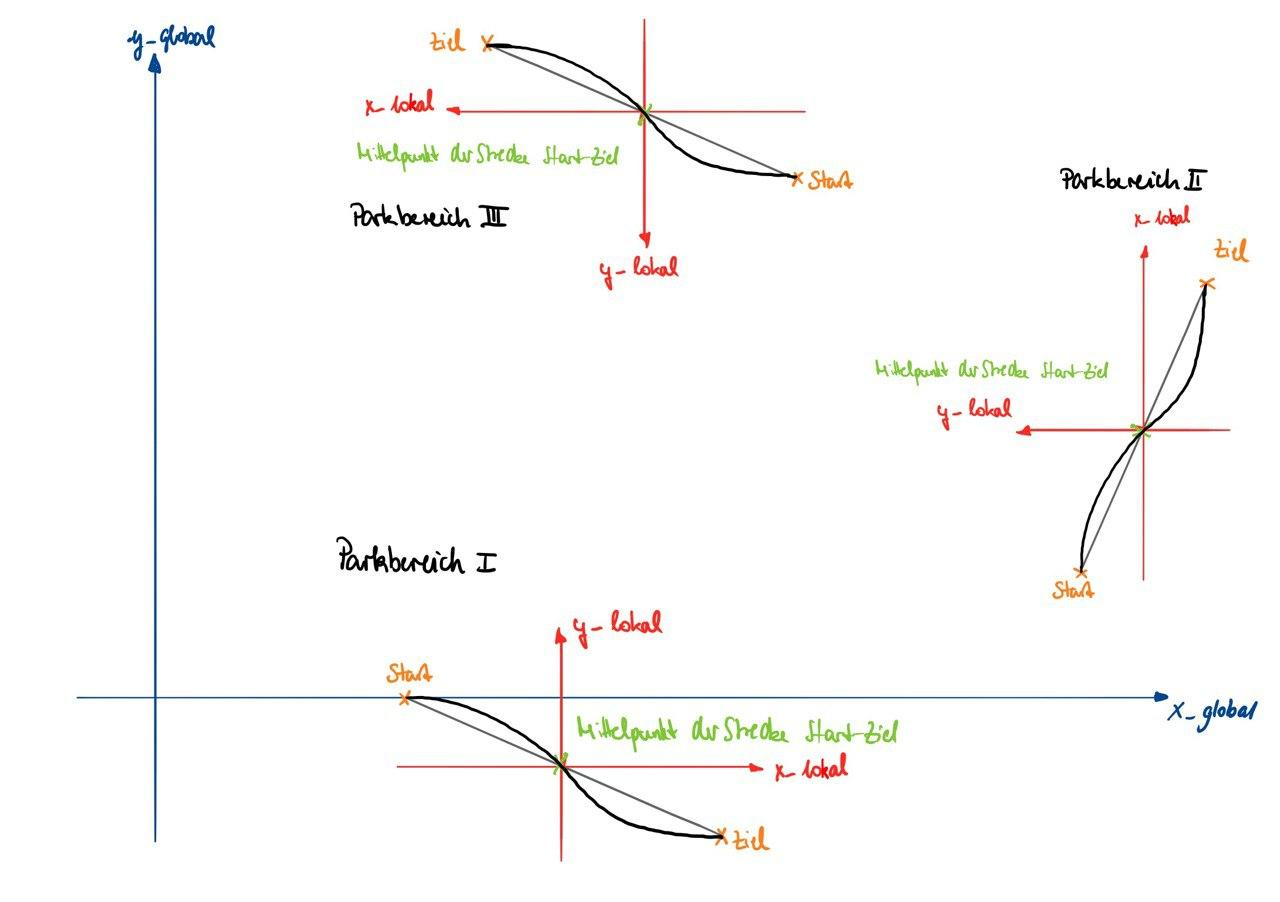
\includegraphics[width=1\textwidth]{SkizzeParklueckenberechung}
	\caption{Skizze für die Parklückenberechung}
	\label{img:grafik-Parkluecke}
\end{figure}
\chapter{Implementierung}

\section{Missionsplaner}
Quellcode hier??!!?
\section{Pfadgenerator}

\chapter{Anmerkungen und Verbesserungsmöglichkeiten}

                               
\end{document}